\documentclass[11pt]{standalone}
\usepackage[usenames]{color} %used for font color
\usepackage{amssymb} %maths
\usepackage{amsmath} %maths
\usepackage[no-math]{fontspec}
\usepackage{unicode-math}
\usepackage{libertinus}
\usepackage{pgf,xcolor}
\definecolor{itwm_blue}{HTML}{005A94}
\definecolor{itwm_red}{HTML}{C00000}
\definecolor{itwm_yellow}{HTML}{e87846}
\usepackage{tikz}
\usepackage{pgfplots}
\pgfplotsset{compat=newest}
\begin{document}
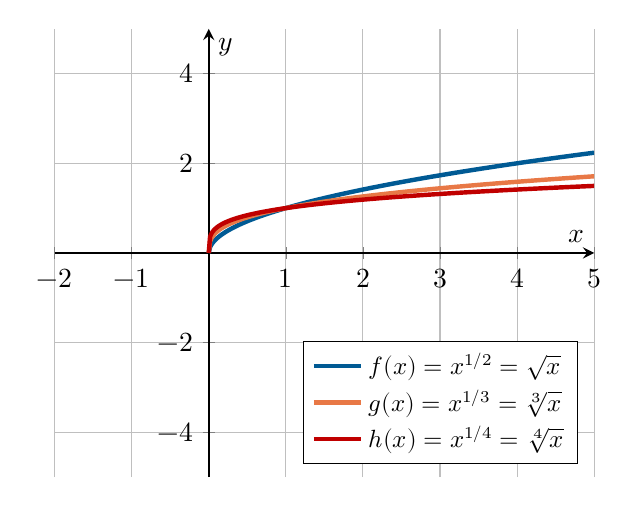
\begin{tikzpicture}
\begin{axis}[
    axis lines = center,
    xlabel = {$x$},
    ylabel = {$y$},
    xmin=-2.0, xmax=5.0,
    ymin=-5.0, ymax=5.0,
    grid = both,
    axis line style={thick},
    legend pos=south east,
    legend style={font=\small},
    legend cell align=left,
    restrict y to domain=-10:10,
    legend entries={$f(x) = x^{1/2}=\sqrt{x}$, $g(x) = x^{1/3}=\sqrt[3]{x}$, $h(x) = x^{1/4}=\sqrt[4]{x}$},
]
    
\addplot[draw=itwm_blue, samples=300, ultra thick, domain=0:5]{ x^(1/2) };
\addplot[draw=itwm_yellow, samples=300, ultra thick, domain=0:5]{ x^(1/3) };
\addplot[draw=itwm_red, samples=300, ultra thick, domain=0:5]{ x^(1/4) };

\end{axis}
\end{tikzpicture}
\end{document}